\documentclass[12pt]{report}
\usepackage{graphicx}
\usepackage{subfig}
\usepackage{listings}
\usepackage{hyperref}
\usepackage{amsmath,amsfonts,amssymb }

\begin{document}
\lstset{language=Python}

\title{Homework 2: Applied Machine Learning}
\author{Tim Delisle and Sam Raudabaugh}
\date{09/29/2015}
\maketitle

\noindent{{\large 1. Face Recognition}}

For this assignment, we investigated a subset of the Yale Face Database. Our goal was to
train a logistic regression classifier that uses eigenfaces to predict which subject is
portrayed in the image.

Once again, we use the \verb+LogisticRegression+ model contained in \verb+scikit-learn+
for this classification. To train the classifier, however, we must first obtain the mean face
$\mu$ from computing the average grayscale intensity of each pixel across the training set.
The mean face is shown in Figure 1.

\begin{figure}
\centering
  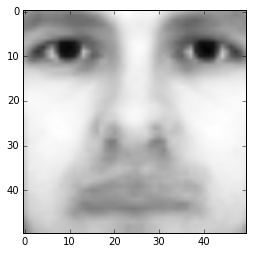
\includegraphics[width=75mm]{figures/mean.png}
\caption{Mean face image}
\end{figure}

We then subtract this from every image and perform Singular Value Decomposition (SVD) on the
dataset to compute the eigenfaces, an example of which is shown in Figure 2. Using the SVD
factors $U$, $\Sigma$, and $V^T$, where $V^T$ is the matrix of eigenfaces, we can construct
low-rank approximations by truncating the number of elements in each factor.

\begin{figure}
\centering
  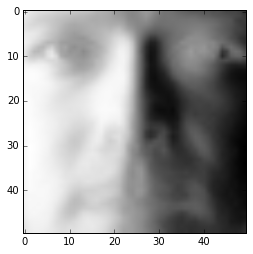
\includegraphics[width=75mm]{figures/eigen.png}
\caption{Example eigenface}
\end{figure}

In Figure 3, a plot of approximation error versus $r$, the number of eigenfaces (first $r$
rows of $V^T$) used in the approximation, is presented. To better understand how our classifier
will perform, we examine the relationship between information loss and the size of the subset of
eigenfaces, and see that the error slope is fairly asymptotic for $r > 100$.

\begin{figure}
\centering
  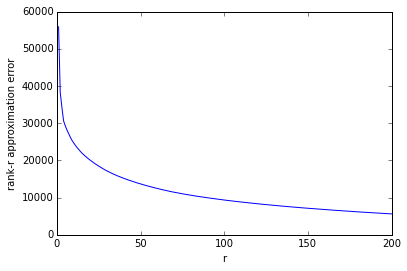
\includegraphics[width=75mm]{figures/error.png}
\caption{Plot of approximation error}
\end{figure}

To use a logistic regression classifier with this data, we build feature matrices out of the
training and test images by projecting them on the subset of eigenfaces (i.e.\ multiplying
$XV^T[:r,:]$). At $r = 10$, the logit model performs with classification accuracy 0.61. Based
on the previous plot of approximation error in Figure 3, we would expect our classifier
to see little improvement in accuracy beyond $r = 100$, and in fact, the plotted accuracy
in Figure 4 shows that this is the case.

\begin{figure}
\centering
  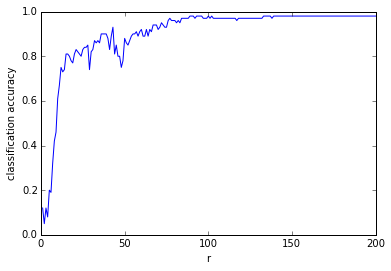
\includegraphics[width=75mm]{figures/accuracy.png}
\caption{Plot of classifier accuracy}
\end{figure}

\hspace{3mm}

\noindent{{\large 2. What's cooking}}

For this problem we joined the What's cooking competition on Kaggle. This problem poses the fun challenge of classifying recipes into cuisines from their underlying ingredients. Our goal was to identify the best model to use to accomplish this classification problem. To accomplish this task we used Scikit Learn's 

We began by exploring the data. The sample data has 39,774 dishes, 20 different cuisines and 6,714 unique ingredients. 

We follow this exploration of the data by with a vectorization of the features. This feature vector is of length 6,714, all possible ingredients. We assign a zero if the ingredient is not present in the recipe and a one if it is. We began by naively implementing our vectorization algorithm by iterating through the vector. We quickly realized that the algorithm was inefficient and therefore decided to implement a mapper where each of the ingredients is used as a key and mapped to a position in the vector (i.e. ``Key" to ``Index"). 

Once vectorized we used our feature matrix to train several different classifiers. We began by testing a naive bayes classifier testing two different underlying distributions, bernoulli and gaussian. To compute the average accuracy for each model we used the cross\_val\_score function provided by scikit learn's cross validation module.

For Gaussian naive bayes, Bernoulli naive bayes and logistic regression we compute average scores of .38, .68 and .78, respectively. The discrepancy between Gaussian and Bernoulli is due to the underlying distribution of the data. If you look at figure 5 which shows the distribution for bacon it is clear that the underlying distribution fits Bernoulli better than Gaussian.

Lastly we submitted our results on Kaggle. Proof of submission is found in figure 6.

\begin{figure}
\centering
  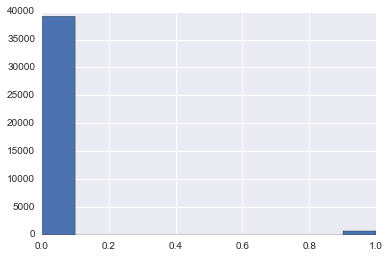
\includegraphics[width=75mm]{figures/bernouli.png}
\caption{Histogram of Bacon}
\end{figure}

\begin{figure}
\centering
  
\includegraphics[width=75mm]{figures/kaggle.png}
\caption{Kaggle Submission}
\end{figure}

\hspace{3mm}

\noindent{{\large 3. Written SVD of rank deficient matrix}}

In this exercise we calculate the singular value decomposition of a matrix as well as an approximation of the original matrix using the largest eigenvalue. We see that this approximation is very close to the original matrix and computed an energy of .908.

\[
M =
\begin{bmatrix}
1 & 2 & 3 \\
3 & 4 & 5 \\
5 & 4 & 3 \\
0 & 2 & 4 \\
1 & 3 & 5
\end{bmatrix}
\]


\[
M^\intercal =
\begin{bmatrix}
1 & 3 & 5 & 0 & 1 \\
2 & 4 & 4 & 2 & 3 \\
3 & 5 & 3 & 4 & 5 
\end{bmatrix}
\]

\[
MM^\intercal =
\begin{bmatrix}
14 & 26 & 22 & 16 & 22 \\
26 & 50 & 46 & 28 & 40 \\
22 & 46 & 50 & 20 & 32 \\
16 & 28 & 20 & 20 & 26 \\
22 & 40 & 32 & 26 & 35
\end{bmatrix}
\]

\[
M^\intercal M =
\begin{bmatrix}
36 & 37 & 38 \\ 
37 & 49 & 61 \\
38 & 61 & 84
\end{bmatrix}
\]

\begin{center}
Eigenvalues for $MM^\intercal$ and $M^\intercal  M$ are the following:

\hspace{3mm}

$\lambda_1 \approx 153.567$

$\lambda_2 \approx 15.433$

$\lambda_3 \approx 0$

$\lambda_4 \approx 0$

$\lambda_5 \approx 0$

\hspace{3mm}

Normalized eigenvectors for $MM^\intercal$ and $M^\intercal  M$ are the following:

\hspace{3mm}

$MM^\intercal$:

$v_1 \approx (0.297696, 0.570509, 0.520742, 0.322578, 0.458985) $

$v_2 \approx (0.159064, -0.0332002, -0.735857, 0.510392, 0.414259) $

$v_3 \approx(-0.912871, 0.182574, 0, 0, 0.365148) $

$v_4 \approx(-0.904534, 0.301511, 0, 0.301511, 0)$

$v_5 \approx(0.784465, -0.588348, 0.196116, 0., 0.) $

\hspace{3mm}

$M^\intercal  M$:

$v_1 \approx (0.409283, 0.56346, 0.717636) $

$v_2 \approx (-0.815978, -0.125885, 0.56421)$

$v_3 \approx (0.408248, -0.816497, 0.408248) $

\end{center}

\[
U =
\begin{bmatrix}
0.297696 & 0.784465  & 0.159064 & -0.912871 & -0.904534 \\
0.570509 & -0.588348  & -0.0332002 & 0.182574 & 0.301511 \\
0.520742 & 0.196116  & -0.735857 & 0 & 0 \\
0.322578 & 0.  & 0.510392 & 0 & 0.301511 \\
0.458985 & 0 & 0.414259 & 0.365148 & 0
\end{bmatrix}
\]

\[
V =
\begin{bmatrix}
0.409283 & -0.815978 & 0.408248 \\
0.56346 & -0.125885 & -0.816497 \\
0.717636 & 0.56421 & 0.408248
\end{bmatrix}
\]

\[
\Sigma =
\begin{bmatrix}
12.3922 & 0 & 0 \\
0 & 3.92849 & 0 \\
0 & 0 & 0 \\
0 & 0 & 0 \\
0 & 0 & 0
\end{bmatrix}
\text{(square root of eigenvalues)}
\]



\[
Aprox =
\begin{bmatrix}
1.509889 & 2.0786628 & 2.64743661 \\
2.89357443 & 3.98358126 & 5.0735881 \\
2.64116728 & 3.63609257 & 4.63101787 \\
1.63609257 & 2.25240715 & 2.86872172 \\
2.32793529 & 3.20486638 & 4.08179747
\end{bmatrix}
\text{(Approximation with first eigenvalue)}
\]

\end{document}
